\documentclass{beamer}

\usepackage[french]{babel}
\usepackage[utf8]{inputenc}
\usepackage{lmodern}
\usepackage{pict2e}
\usepackage{graphicx}
\usepackage{schemabloc}
\usetikzlibrary{quotes}
\tikzset{%
  node distance=5cm,
  every edge quotes/.append style={midway, below},
}

\usetheme{Madrid}

\definecolor{InvisibleRed}{rgb}{0.92, 0.9, 0.9}
\definecolor{InvisibleGreen}{rgb}{0.9, 0.92, 0.9}
\definecolor{InvisibleBlue}{rgb}{0.9, 0.9, 0.92}

\definecolor{LightBlue}{rgb}{0.4, 0.55, 0.65}

\definecolor{MediumRed}{rgb}{0.92549, 0.34509, 0.34509}
\definecolor{MediumGreen}{rgb}{0.36862, 0.66666, 0.65882}
\definecolor{MediumBlue}{rgb}{0.01176, 0.31372, 0.43529}

\definecolor{DarkBlue}{rgb}{0.05, 0.15, 0.3} 

\usecolortheme[named=LightBlue]{structure}

\setbeamercolor{palette primary}{bg=DarkBlue,fg=white}
\setbeamercolor{palette secondary}{bg=MediumBlue,fg=white}
\setbeamercolor{palette tertiary}{bg=LightBlue,fg=white}
\setbeamercolor{block title}{bg=MediumBlue}
\setbeamercolor{block body}{bg=InvisibleBlue}
\setbeamercolor{block title example}{bg=MediumGreen}
\setbeamercolor{block body example}{bg=InvisibleGreen}
\setbeamercolor{block title alerted}{bg=MediumRed}
\setbeamercolor{block body alerted}{bg=InvisibleRed}






%Information to be included in the title page:
\title[Astre - Projet] %optional
{Modélisation et vérification de systèmes concurrents}

\subtitle{Architecture multiprocesseur à mémoire partagée}

\author[K.~Ly, M.~Eliet] % (optional, for multiple authors)
{Kimmeng Ly \and Max Eliet}

\institute[Sorbonne Université] % (optional)
{
  Sorbonne Université Sciences
}

\date[\today] % (optional)
{Encadrante : E.~Encrenaz}



\begin{document}

\frame{\titlepage}

\begin{frame}
\frametitle{Introduction}
\onslide<1->{
On considère un système multiprocesseur à mémoire partagée. Le système est muni d’une hiérarchie mémoire à deux niveaux :
}
\onslide<2->{
    \begin{block}{Mémoire centrale}
        Stocke les instructions, données, pile des programmes en cours d’exécution et du système d’exploitation.
    \end{block}
}

\onslide<3>{
    \begin{block}{Caches privés}
        Associés à chaque processeur et comprennent deux parties distinctes :
        \begin{itemize}
            \item Caches d'instructions
            \item Caches de données
        \end{itemize}
    \end{block}
}
\end{frame}

%------------------------------------------------

\begin{frame}{Etude du protocole et des accès aux données partagées}
    \textbf{Cas monoprocesseur : effet cache}
    \begin{columns}[c] % The "c" option specifies centered vertical alignment while the "t" option is used for top vertical alignment

        \column{.3\textwidth} % Left column and width
        \textbf{P1a : }

        \column{.6\textwidth} % Right column and width
        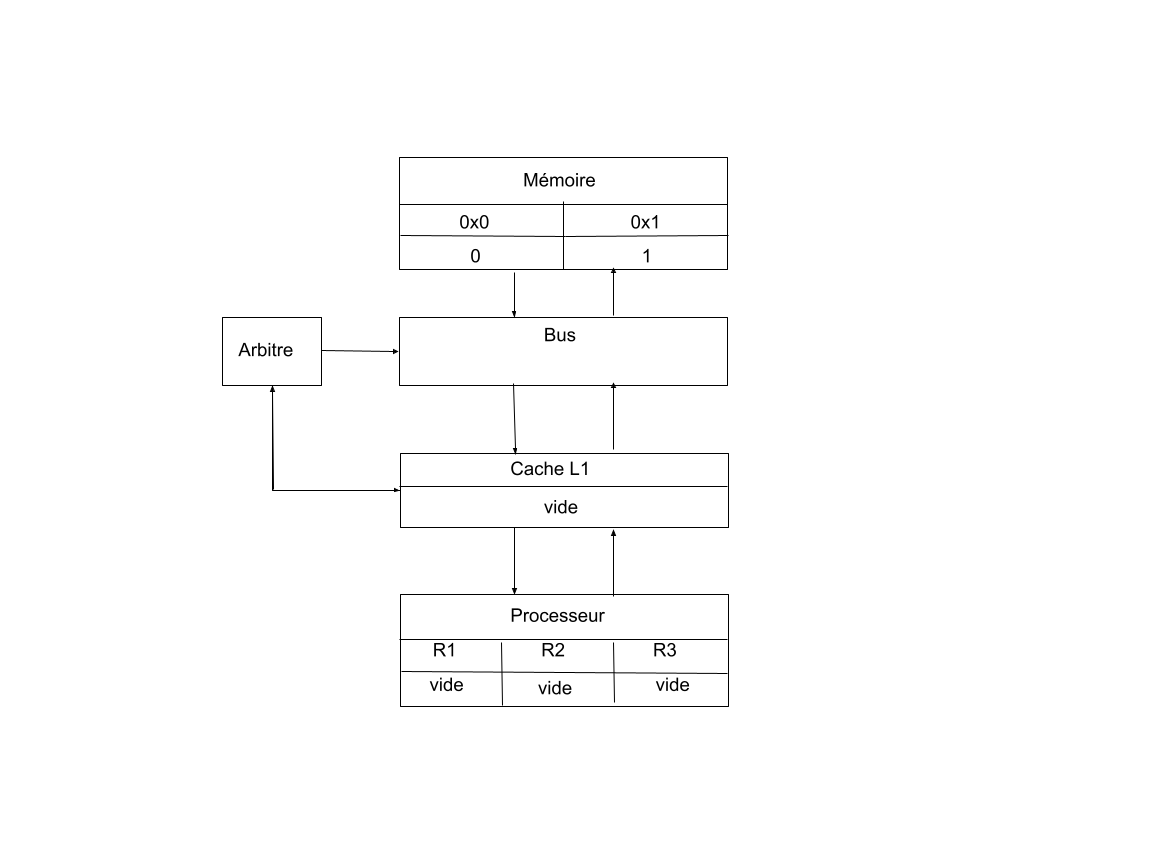
\includegraphics[scale=0.28]{f0.png}
        
    \end{columns}
\end{frame}

\begin{frame}{Etude du protocole et des accès aux données partagées}
    \addtocounter{framenumber}{-1}
    \textbf{Cas monoprocesseur : effet cache}
    \begin{columns}[c] % The "c" option specifies centered vertical alignment while the "t" option is used for top vertical alignment

        \column{.3\textwidth} % Left column and width
        \textbf{P1a : }
        \begin{itemize}
            \item ld R1, [0]
        \end{itemize}

        \column{.6\textwidth} % Right column and width
        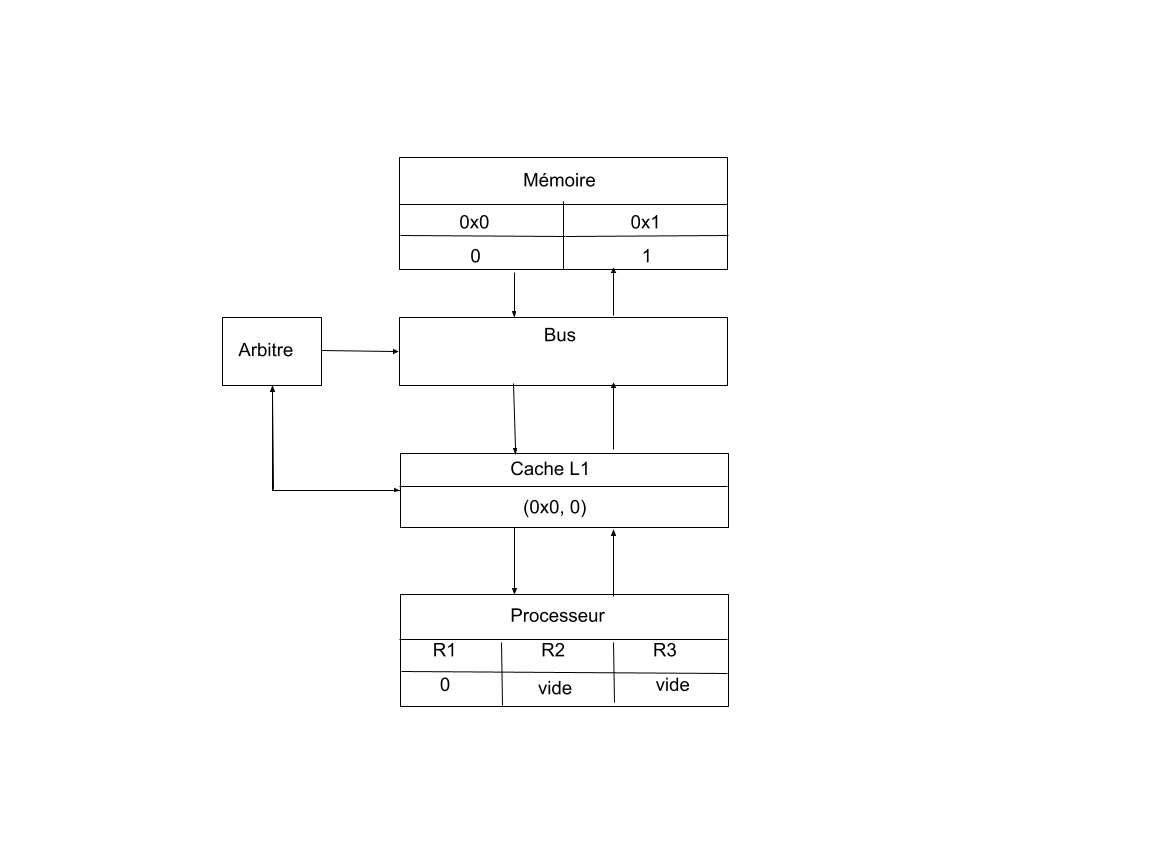
\includegraphics[scale=0.28]{f1.png}
        
    \end{columns}
\end{frame}

\begin{frame}{Etude du protocole et des accès aux données partagées}
    \addtocounter{framenumber}{-1}
    \textbf{Cas monoprocesseur : effet cache}
    \begin{columns}[c] % The "c" option specifies centered vertical alignment while the "t" option is used for top vertical alignment

        \column{.3\textwidth} % Left column and width
        \textbf{P1a : }
        \begin{itemize}
            \item ld R1, [0]
            \item add R1, R1, 1
        \end{itemize}

        \column{.6\textwidth} % Right column and width
        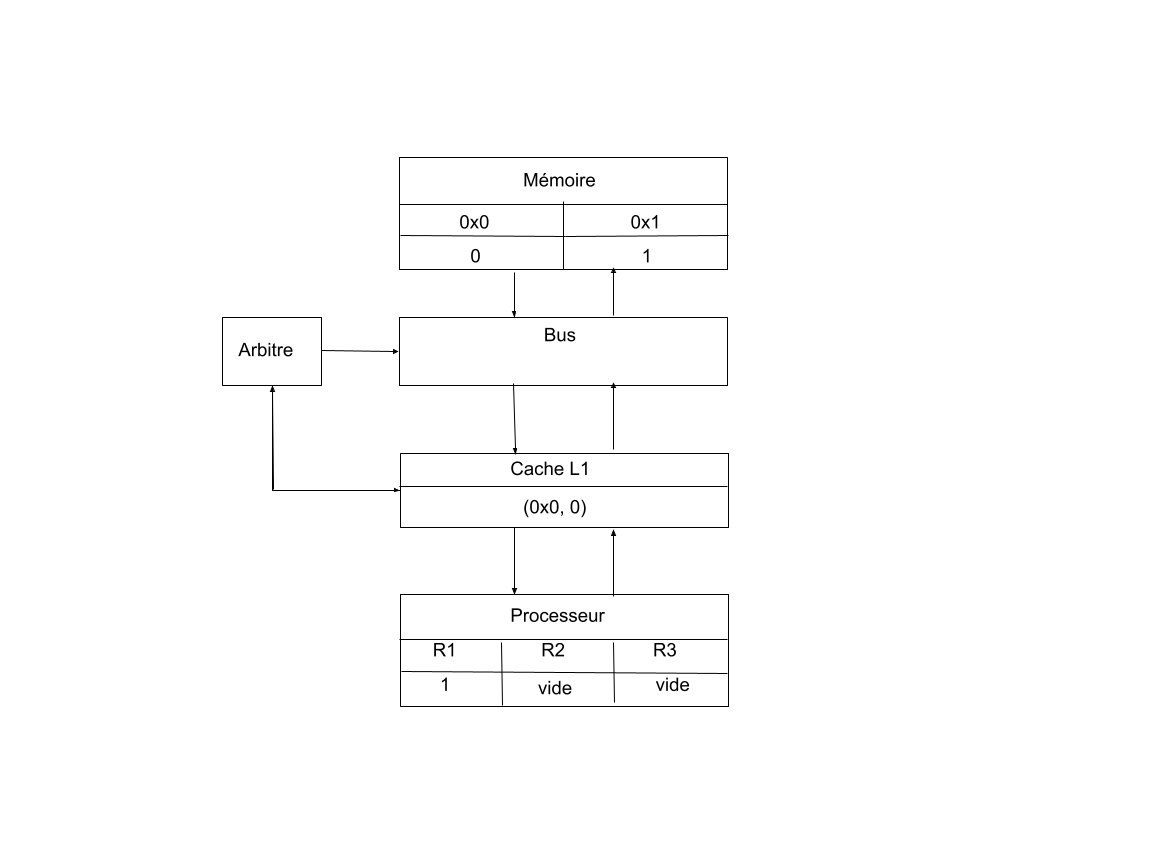
\includegraphics[scale=0.28]{f2.png}
        
    \end{columns}
\end{frame}

\begin{frame}{Etude du protocole et des accès aux données partagées}
    \addtocounter{framenumber}{-1}
    \textbf{Cas monoprocesseur : effet cache}
    \begin{columns}[c] % The "c" option specifies centered vertical alignment while the "t" option is used for top vertical alignment

        \column{.3\textwidth} % Left column and width
        \textbf{P1a : }
        \begin{itemize}
            \item ld R1, [0]
            \item add R1, R1, 1
            \item  st R1, [1]
        \end{itemize}

        \column{.6\textwidth} % Right column and width
        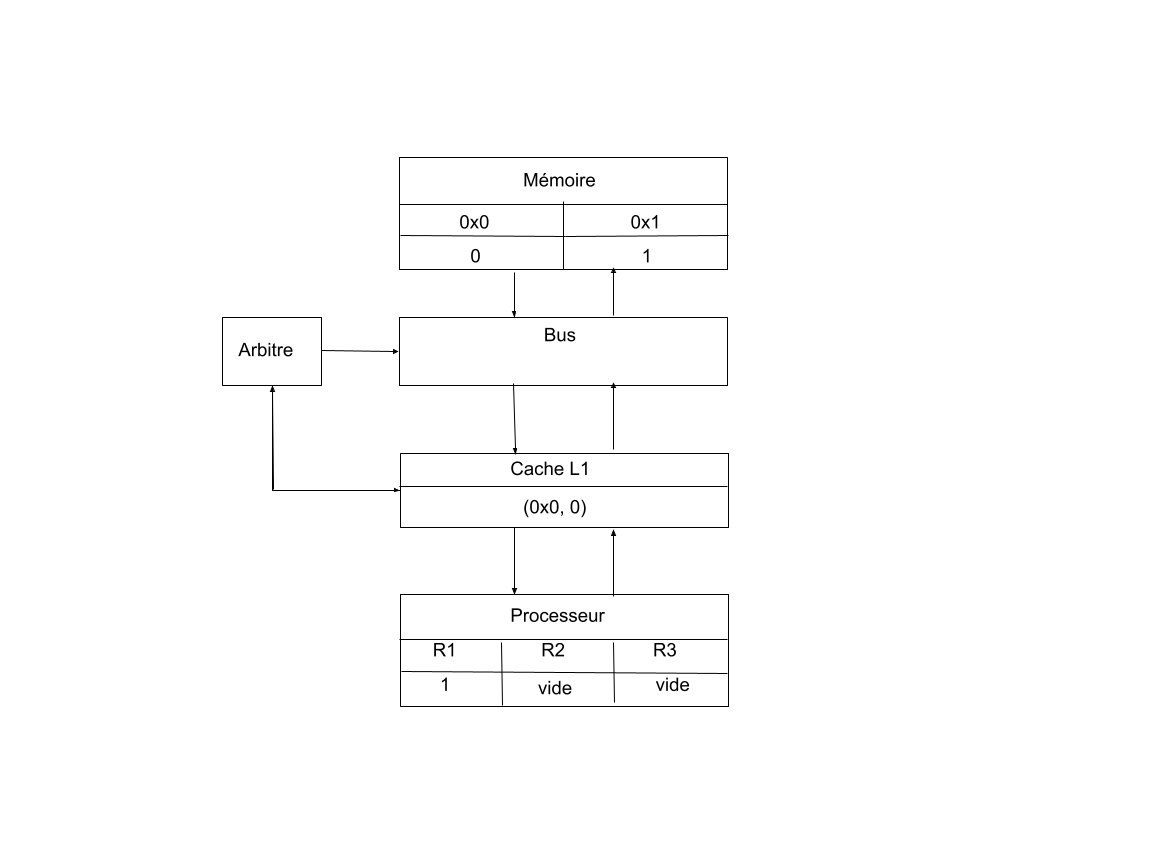
\includegraphics[scale=0.28]{f3.png}
        
    \end{columns}
\end{frame}

\begin{frame}{Etude du protocole et des accès aux données partagées}
    \addtocounter{framenumber}{-1}
    \textbf{Cas monoprocesseur : effet cache}
    \begin{columns}[c] % The "c" option specifies centered vertical alignment while the "t" option is used for top vertical alignment

        \column{.3\textwidth} % Left column and width
        \textbf{P1a : }
        \begin{itemize}
            \item ld R1, [0]
            \item add R1, R1, 1
            \item  st R1, [1]
            \item  ld R2, [0]
        \end{itemize}

        \column{.6\textwidth} % Right column and width
        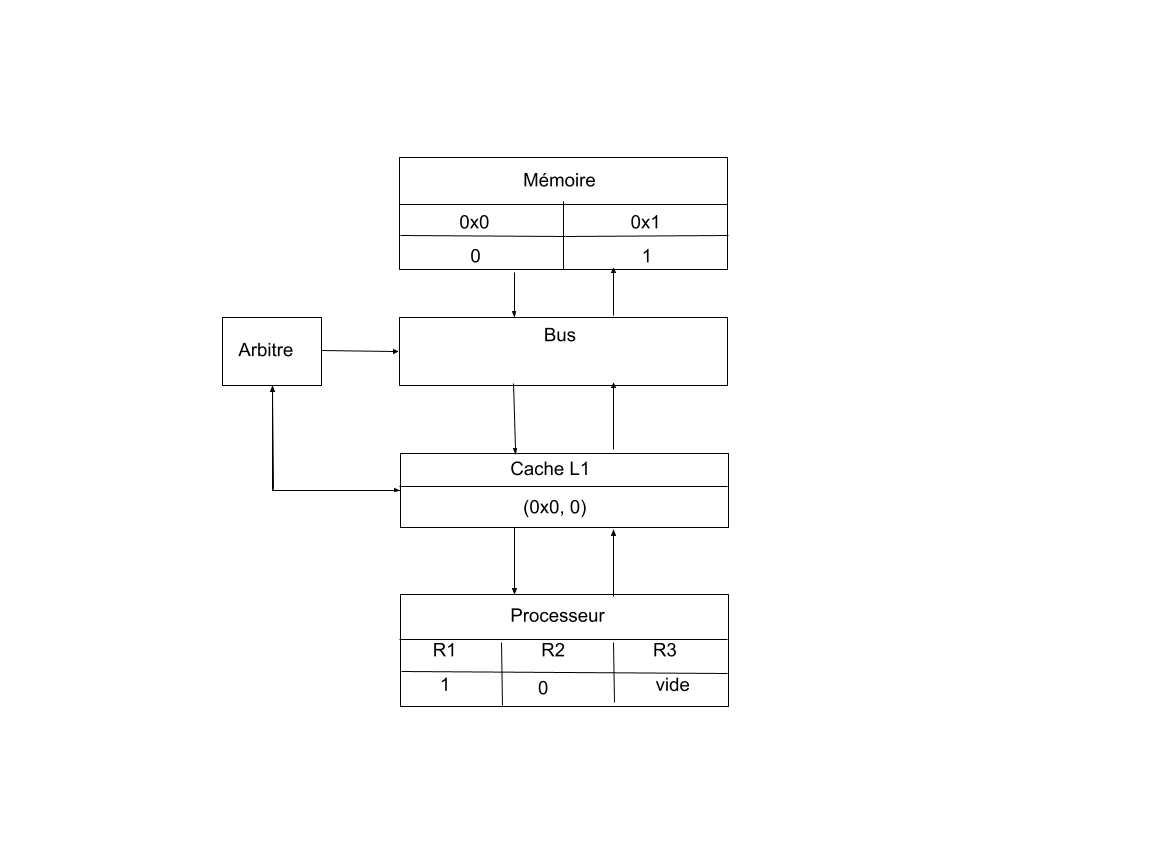
\includegraphics[scale=0.28]{f4.png}
        
    \end{columns}
\end{frame}

\begin{frame}{Etude du protocole et des accès aux données partagées}
    \addtocounter{framenumber}{-1}
    \textbf{Cas monoprocesseur : effet cache}
    \begin{columns}[c] % The "c" option specifies centered vertical alignment while the "t" option is used for top vertical alignment

        \column{.3\textwidth} % Left column and width
        \textbf{P1a : }
        \begin{itemize}
            \item ld R1, [0]
            \item add R1, R1, 1
            \item  st R1, [1]
            \item  ld R2, [0]
            \item add R2, R2, 1
        \end{itemize}

        \column{.6\textwidth} % Right column and width
        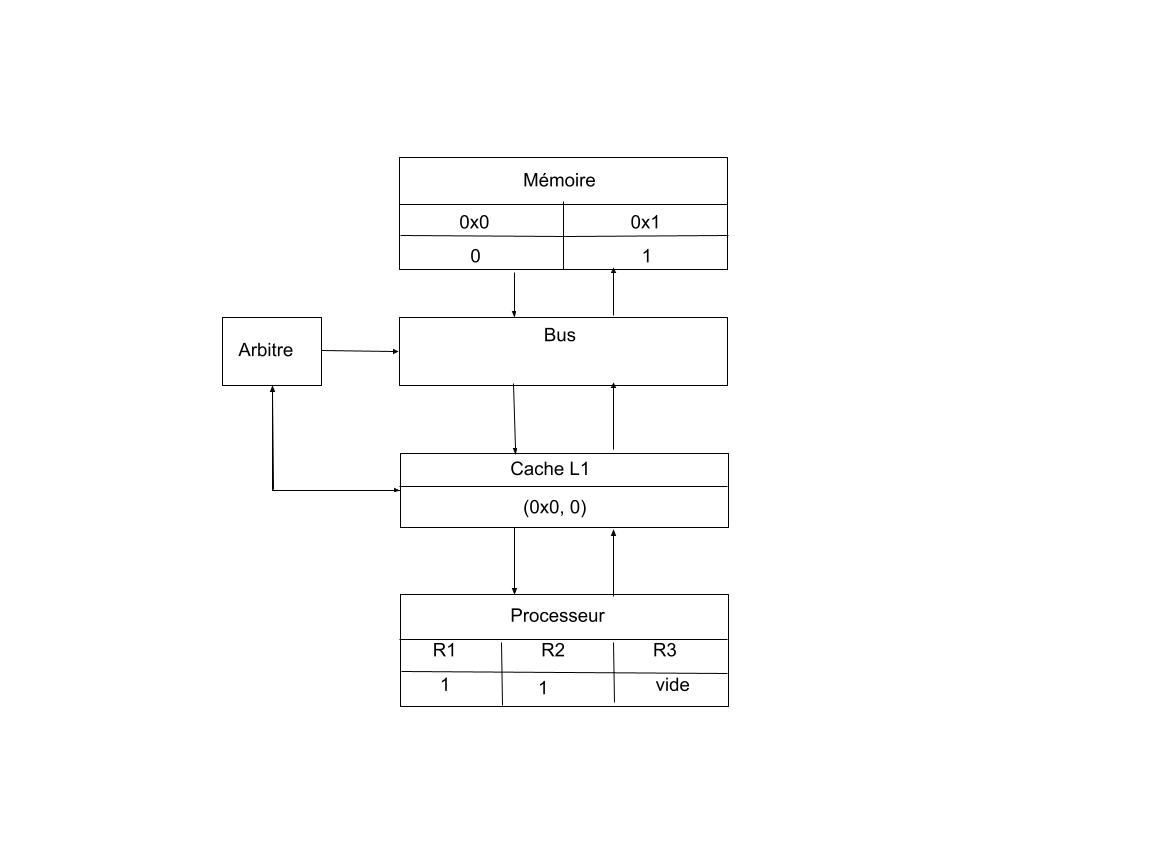
\includegraphics[scale=0.28]{f5.png}
        
    \end{columns}
\end{frame}

\begin{frame}{Etude du protocole et des accès aux données partagées}
    \addtocounter{framenumber}{-1}
    \textbf{Cas monoprocesseur : effet cache}
    \begin{columns}[c] % The "c" option specifies centered vertical alignment while the "t" option is used for top vertical alignment

        \column{.3\textwidth} % Left column and width
        \textbf{P1a : }
        \begin{itemize}
            \item ld R1, [0]
            \item add R1, R1, 1
            \item  st R1, [1]
            \item  ld R2, [0]
            \item add R2, R2, 1
            \item st R2, [0]
        \end{itemize}

        \column{.6\textwidth} % Right column and width
        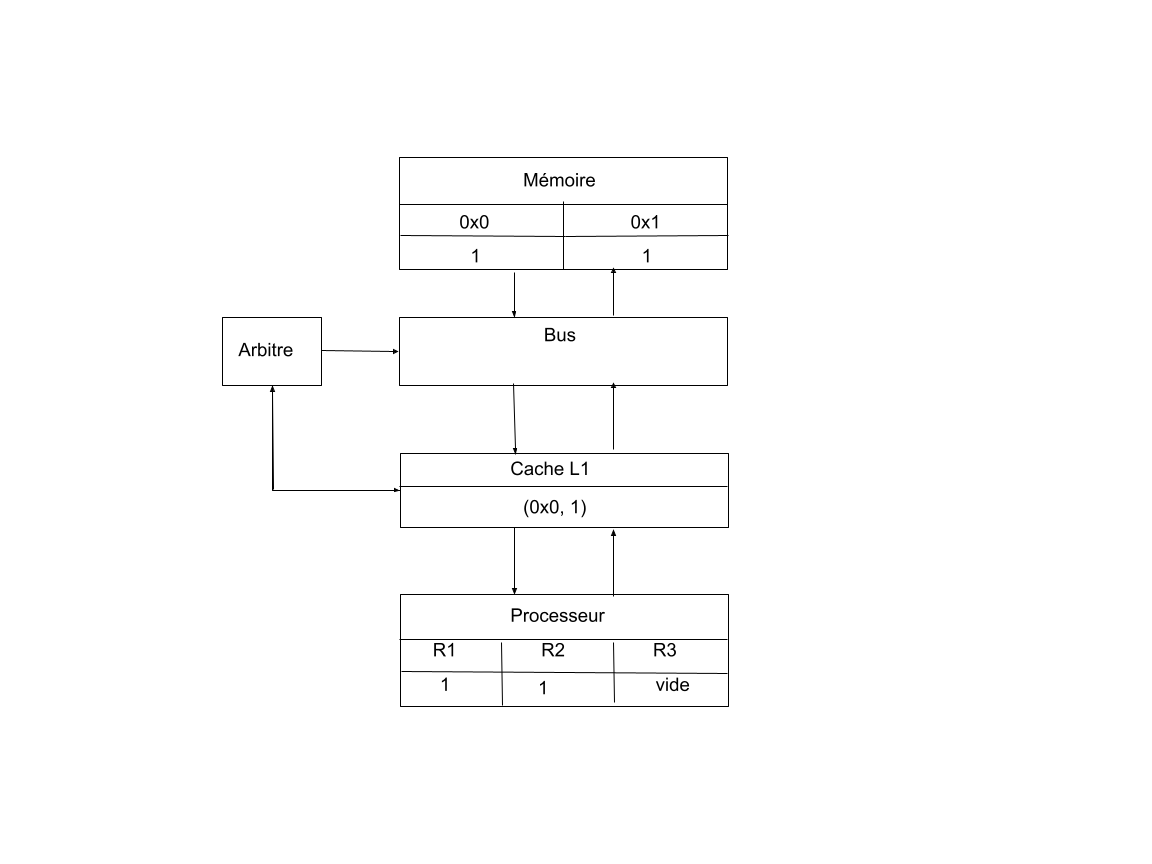
\includegraphics[scale=0.28]{f6.png}
        
    \end{columns}
\end{frame}

%------------------------------P1b-----------------------------------------------------------------------
%-----------------------------------------------------------------------------------------------------
%-----------------------------------------------------------------------------------------------------

\begin{frame}{Etude du protocole et des accès aux données partagées}
    \textbf{Cas monoprocesseur : éviction du cache / écriture write-trough}
    \begin{columns}[c] % The "c" option specifies centered vertical alignment while the "t" option is used for top vertical alignment

        \column{.3\textwidth} % Left column and width
        \textbf{P1b : }

        \column{.6\textwidth} % Right column and width
        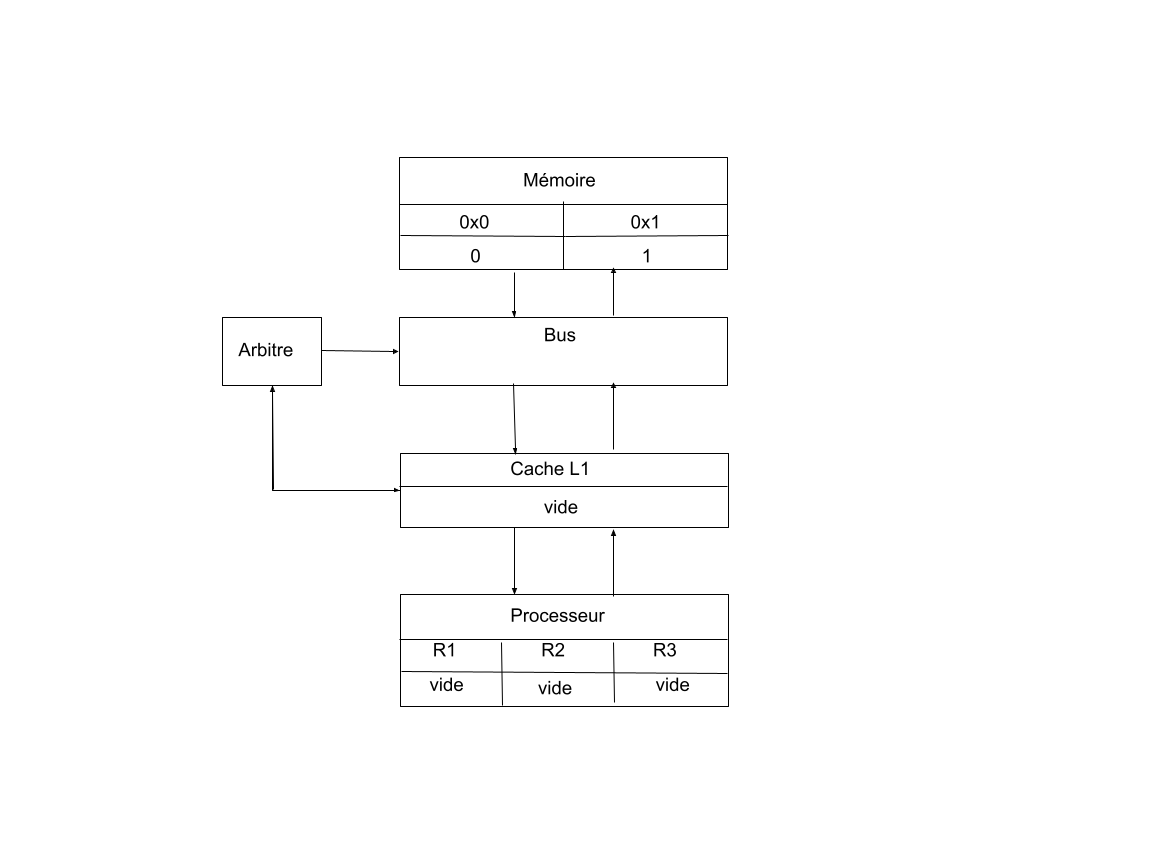
\includegraphics[scale=0.28]{f0.png}
        
    \end{columns}
\end{frame}

\begin{frame}{Etude du protocole et des accès aux données partagées}
    \addtocounter{framenumber}{-1}
    \textbf{Cas monoprocesseur : éviction du cache / écriture write-trough}
    \begin{columns}[c] % The "c" option specifies centered vertical alignment while the "t" option is used for top vertical alignment

        \column{.3\textwidth} % Left column and width
        \textbf{P1b : }
        \begin{itemize}
            \item ld R1, [0]
        \end{itemize}

        \column{.6\textwidth} % Right column and width
        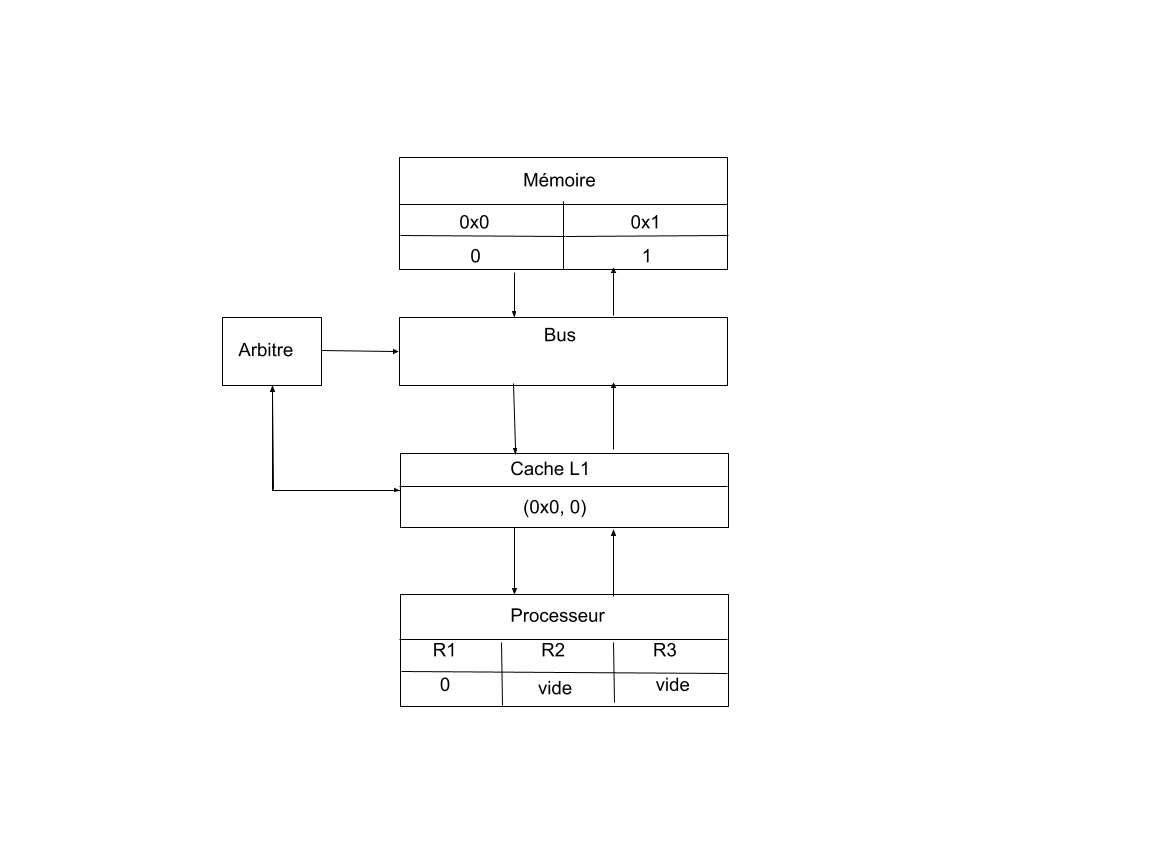
\includegraphics[scale=0.28]{f1.png}
        
    \end{columns}
\end{frame}

\begin{frame}{Etude du protocole et des accès aux données partagées}
    \addtocounter{framenumber}{-1}
    \textbf{Cas monoprocesseur : éviction du cache / écriture write-trough}
    \begin{columns}[c] % The "c" option specifies centered vertical alignment while the "t" option is used for top vertical alignment

        \column{.3\textwidth} % Left column and width
        \textbf{P1b : }
        \begin{itemize}
            \item ld R1, [0]
            \item ld R2, [1]
        \end{itemize}

        \column{.6\textwidth} % Right column and width
        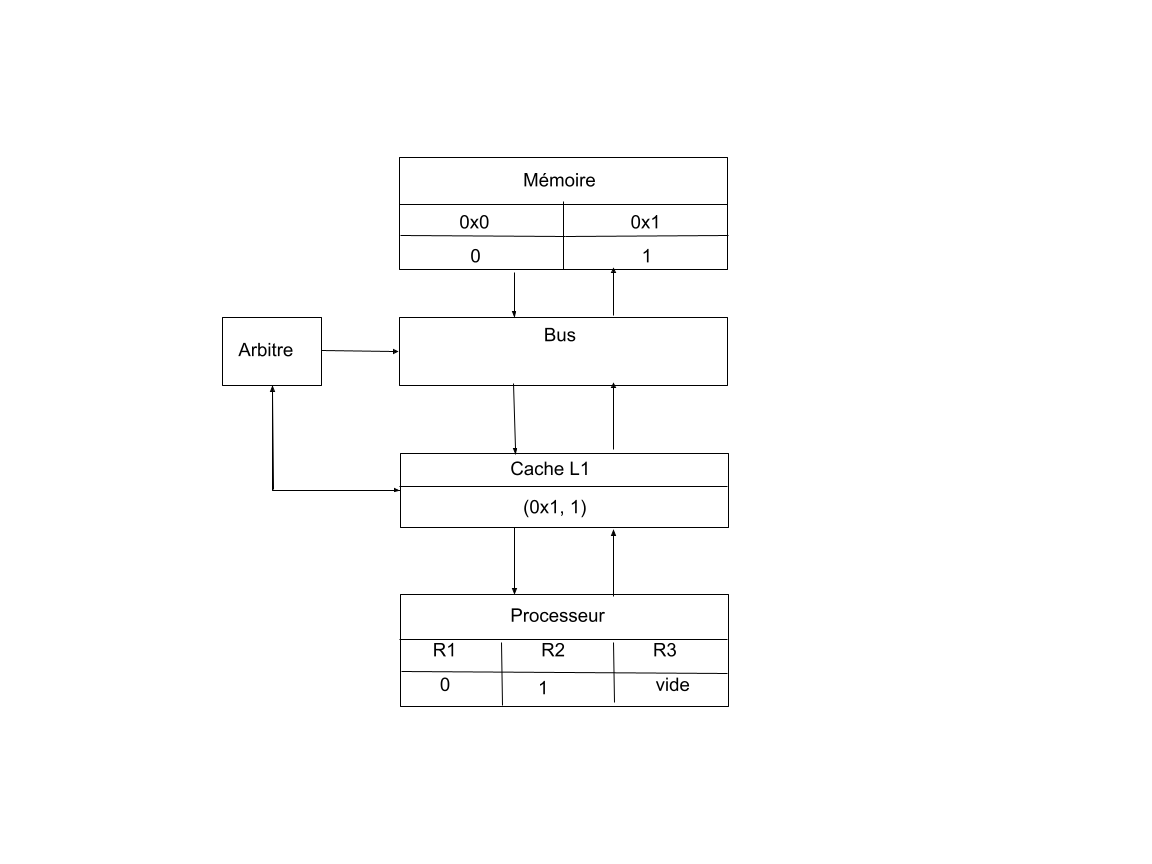
\includegraphics[scale=0.28]{f2b.png}
        
    \end{columns}
\end{frame}

\begin{frame}{Etude du protocole et des accès aux données partagées}
    \addtocounter{framenumber}{-1}
    \textbf{Cas monoprocesseur : éviction du cache / écriture write-trough}
    \begin{columns}[c] % The "c" option specifies centered vertical alignment while the "t" option is used for top vertical alignment

        \column{.3\textwidth} % Left column and width
        \textbf{P1b : }
        \begin{itemize}
            \item ld R1, [0]
            \item ld R2, [1]
            \item add R3, R1, R2
        \end{itemize}

        \column{.6\textwidth} % Right column and width
        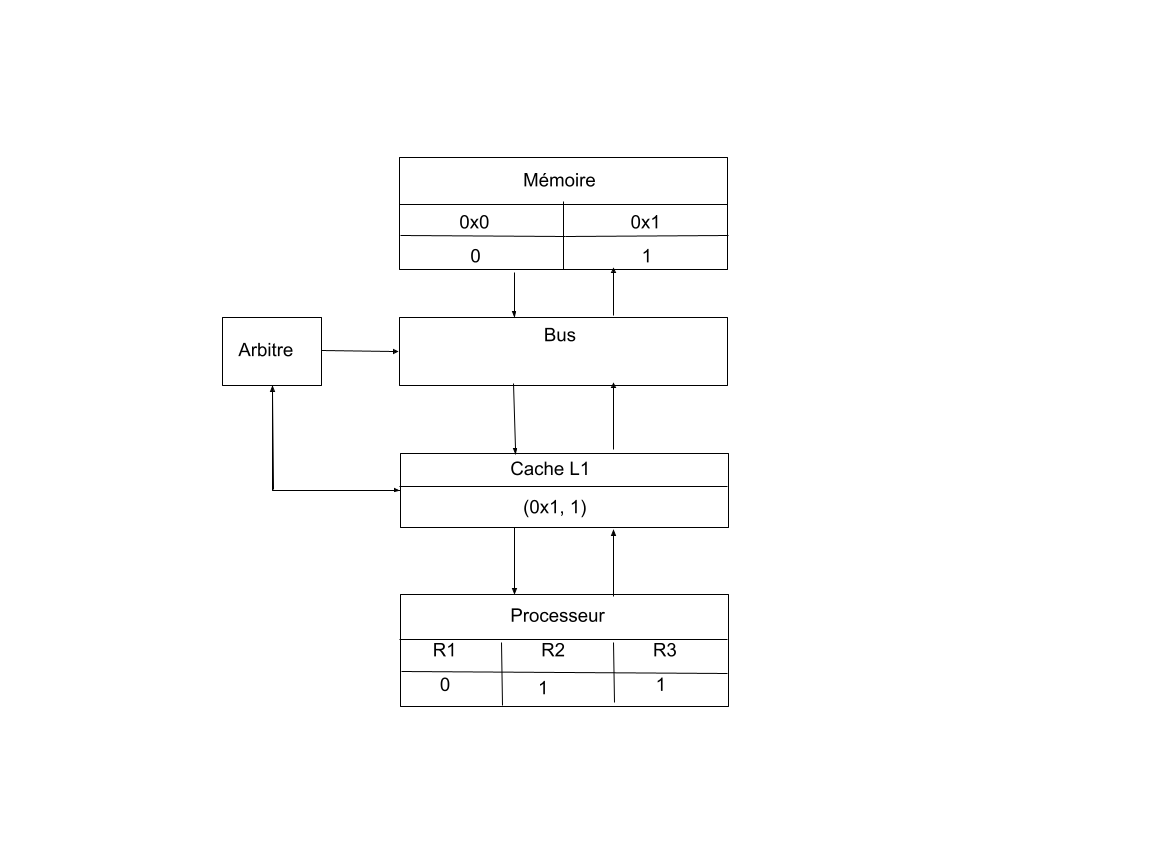
\includegraphics[scale=0.28]{f3b.png}
        
    \end{columns}
\end{frame}

\begin{frame}{Etude du protocole et des accès aux données partagées}
    \addtocounter{framenumber}{-1}
    \textbf{Cas monoprocesseur : éviction du cache / écriture write-trough}
    \begin{columns}[c] % The "c" option specifies centered vertical alignment while the "t" option is used for top vertical alignment

        \column{.3\textwidth} % Left column and width
        \textbf{P1b : }
        \begin{itemize}
            \item ld R1, [0]
            \item ld R2, [1]
            \item add R3, R1, R2
            \item st R3, [0] 
        \end{itemize}

        \column{.6\textwidth} % Right column and width
        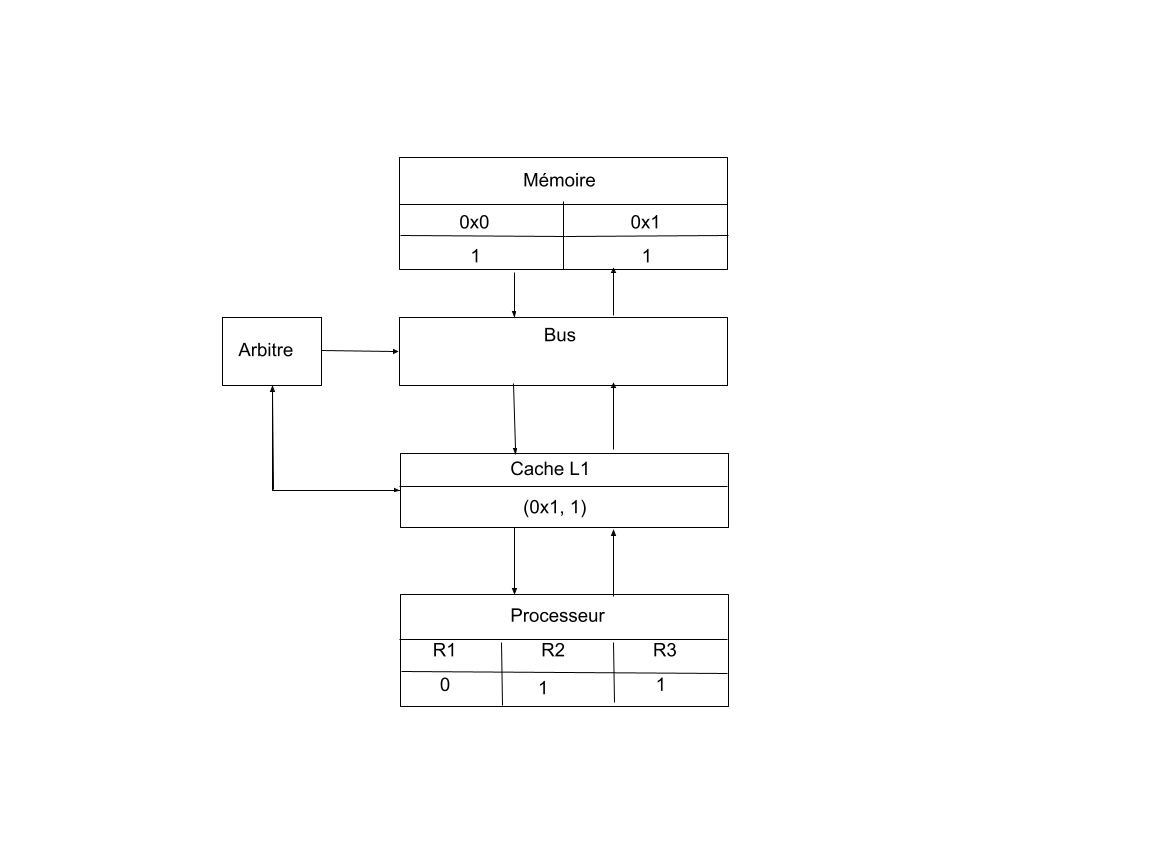
\includegraphics[scale=0.28]{f4b.png}
        
    \end{columns}
\end{frame}

%------------------------------Multiprocesseurs-----------------------------------------------------------------------
%-----------------------------------------------------------------------------------------------------
%-----------------------------------------------------------------------------------------------------

\begin{frame}{Etude du protocole et des accès aux données partagées}
    \textbf{Cas multiprocesseur : partage en lecture / une écriture}
    \begin{columns}[c] % The "c" option specifies centered vertical alignment while the "t" option is used for top vertical alignment

        \column{.3\textwidth} % Left column and width
        \textbf{P1a : }
        \begin{itemize}
            \item ld R1, [0]
        \end{itemize}

        \textbf{P2a : }
        \begin{itemize}
            \item ld R1, [0]
        \end{itemize}

        \textbf{P3a : }
        \begin{itemize}
            \item inactif
        \end{itemize}

        \column{.6\textwidth} % Right column and width
        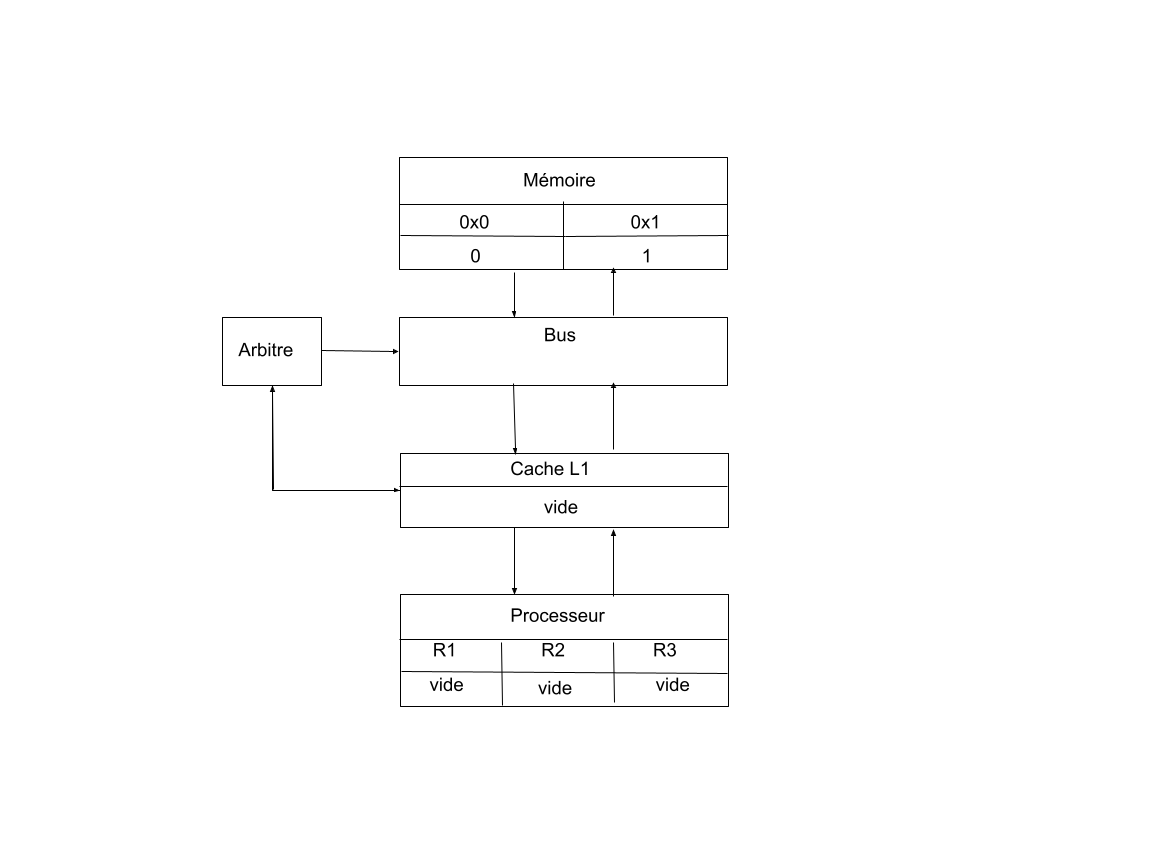
\includegraphics[scale=0.28]{f0.png}
        
    \end{columns}
\end{frame}

\end{document}
